\documentclass[10pt]{article}
\usepackage[paperheight=303mm,paperwidth=431.9mm,
top=2.5cm, bottom=3cm,right=2.5cm, left=3.5cm]{geometry}
\usepackage{graphicx}
\usepackage{amssymb}
\usepackage{epstopdf}
\DeclareGraphicsRule{.tif}{png}{.png}{`convert #1 `dirname #1`/`basename #1 .tif`.png}
\usepackage{blindtext}
\usepackage[T1]{fontenc}
\usepackage[default]{opensans}
\usepackage{graphicx}
\usepackage{pbox}
\usepackage{setspace}
\usepackage[misc]{ifsym}
\usepackage{microtype}
\usepackage{tikz,ifthen}
\usepackage{xcolor}
\usepackage{pgfplots}
\usepackage{colortbl}
\usepackage{subcaption}

\begin{document}
\thispagestyle{empty}

\noindent{\large\bfseries Cover figures}

 \begin{figure}
     \begin{subfigure}[b]{0.1\textwidth}
          \centering
          \resizebox{\linewidth}{!}{
          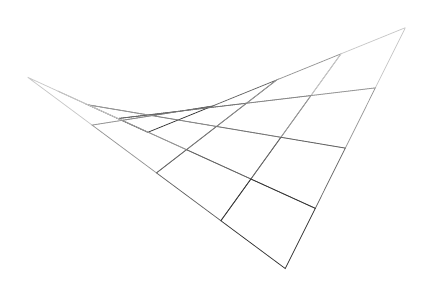
\begin{tikzpicture}[scale=0.7]
	\begin{axis}[
		axis lines=none,
		samples=5, domain=-4:4,
		xtick=data, ytick=data,
		colormap/blackwhite,
	]
		\addplot3[mesh] {x*y};
	\end{axis}
\end{tikzpicture}
          }
          \caption{Frontcover left}
          \label{fig:A}
     \end{subfigure}
     \begin{subfigure}[b]{0.10\textwidth}
          \centering
          \resizebox{\linewidth}{!}{
          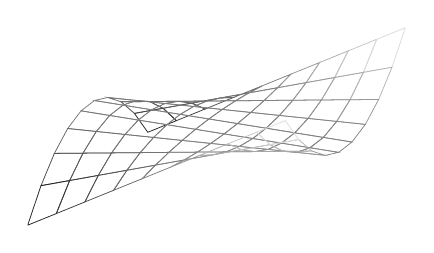
\begin{tikzpicture}[scale=0.7]
	\begin{axis}[
		axis lines=none,
		samples=10, domain=-4:4,
		xtick=data, ytick=data,
		colormap/blackwhite,
	]
		\addplot3[mesh] {x*y^2};
	\end{axis}
\end{tikzpicture}
          }
          \caption{Frontcover center}
          \label{fig:B}
     \end{subfigure}
     \begin{subfigure}[b]{0.10\textwidth}
          \centering
          \resizebox{\linewidth}{!}{
          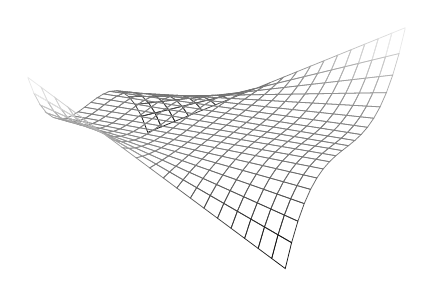
\begin{tikzpicture}[scale=0.7]
	\begin{axis}[
		axis lines=none,
		samples=20, domain=-4:4,
		xtick=data, ytick=data,
		colormap/blackwhite,
	]
		\addplot3[mesh] {x*y^3};
	\end{axis}
\end{tikzpicture}
          }
          \caption{Frontcover right}
          \label{fig:C}
     \end{subfigure}
     
          \begin{subfigure}[b]{0.10\textwidth}
          \centering
          \resizebox{\linewidth}{!}{
          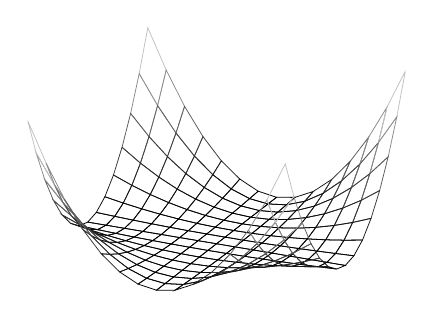
\begin{tikzpicture}[scale=0.7]
	\begin{axis}[
		axis lines=none,
		samples=15, domain=-4:4,
		xtick=data, ytick=data,
		colormap/blackwhite,
	]
		\addplot3[mesh] {x^2*y^2};
	\end{axis}
\end{tikzpicture}
          }
          \caption{Backcover}
          \label{fig:D}
     \end{subfigure}
 \end{figure}

\vspace{0.5cm}
\noindent The cover figures are random functions plotted in TikZ, and are unrelated to the\\thesis topic. The functions are:\\
\vspace{0.5cm}

\noindent (a) Frontcover left: $f(x,y)=x\times y$, for $x$ and $y$ $\in [-4,4]$;\\
(b) Frontcover center: $g(x,y)=x\times y^2$, for $x$ and $y$ $\in [-4,4]$;\\
(c) Frontcover right: $h(x,y)=x\times y^3$, for $x$ and $y$ $\in [-4,4]$ and\\
(d) Backcover: $i(x,y)=x^2\times y^2$, for $x$ and $y$ $\in [-4,4]$.

\end{document} 
